\documentclass[border=10pt]{standalone}
\usepackage{tikz}
\usetikzlibrary{arrows, decorations.markings, calc, fadings, decorations.pathreplacing, patterns, decorations.pathmorphing, positioning}
\tikzstyle{every path}=[line width=1.2pt]

\begin{document}
\newcommand{\bigf}[1]{\Large{#1}} % Ký hiệu cho máy phát
\newcommand{\bbigf}[1]{\huge{#1}} % Tên của các phần tử
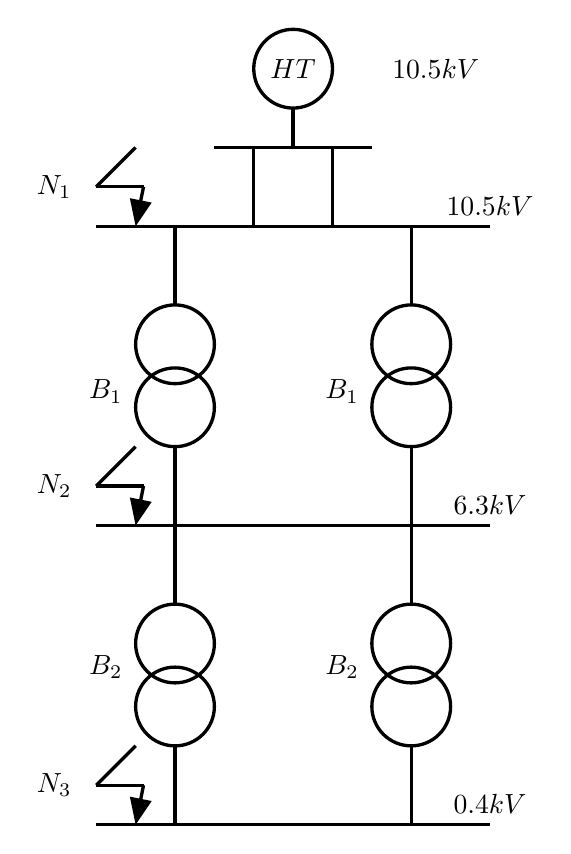
\begin{tikzpicture}[>=triangle 45]
%\draw[color=blue] (-2,-2) grid (11,11); %Tạo lưới
\draw (-1,0) -- (4,0); % Nối 2 máy biến áp B2

\draw (0,0) -- (0,1);
\draw (0,1.5) circle (.5); %Vẽ máy biến áp B2
\draw (0,2.3) circle (.5);
\draw (0,2.8) -- (0,3.8);
\draw (0,2) node[left=15pt] {\bigf{$B_2$}};

\draw (3,0) -- (3,1);%
\draw (3,1.5) circle (.5); %Vẽ máy biến áp B2
\draw (3,2.3) circle (.5);
\draw (3,2.8) -- (3,3.8);
\draw (3,2) node[left=15pt] {\bigf{$B_2$}};

\draw (-1,3.8) -- (4,3.8); % Nối 2 máy biến áp B2

\draw (0,3.8) -- (0,4.8);
\draw (0,5.3) circle (.5); %Vẽ máy biến áp B1
\draw (0,6.1) circle (.5);
\draw (0,6.6) -- (0,7.6);
\draw (0,5.5) node[left=15pt] {\bigf{$B_1$}};

\draw (3,3.8) -- (3,4.8);
\draw (3,5.3) circle (.5); %Vẽ máy biến áp B1
\draw (3,6.1) circle (.5);
\draw (3,6.6) -- (3,7.6);
\draw (3,5.5) node[left=15pt] {\bigf{$B_1$}};

\draw (-1,7.6) -- (4,7.6); % Nối 2 máy biến áp B1

\draw (1,7.6) -- (1,8.6); %Đường dây kép
\draw (2,7.6) -- (2,8.6);
\draw (.5,8.6) -- (2.5,8.6);

\draw (1.5,8.6) -- (1.5,9.1); % Nối đường dây kép với hệ thống

\draw (1.5,9.6) circle (0.5) node {\bigf{$HT$}}; %Vẽ hệ thống
\draw (4,9.6) node[left] {\bigf{$10.5kV$}};

%Điện áp thanh cái
\draw (4,0) node[above] {\bigf{$0.4kV$}};
\draw (4,3.8) node[above] {\bigf{$6.3kV$}};
\draw (4,7.6) node[above] {\bigf{$10.5kV$}};

%Vẽ điểm ngắn mạch
\draw (-0.5,8.6) -- (-1,8.1);	% Tại N1
\draw (-1,8.1) -- (-0.4,8.1);
\draw[->] (-0.4,8.1) -- (-.5,7.6);
\draw (-1,8.1) node[left=5pt] {\bigf{$N_1$}};

\draw (-0.5,4.8) -- (-1,4.3);	% Tại N2
\draw (-1,4.3) -- (-0.4,4.3);
\draw[->] (-0.4,4.3) -- (-.5,3.8);
\draw (-1,4.3) node[left=5pt] {\bigf{$N_2$}};

\draw (-0.5,1) -- (-1,.5);	% Tại N3
\draw (-1,.5) -- (-0.4,.5);
\draw[->] (-0.4,.5) -- (-.5,0);
\draw (-1,.5) node[left=5pt] {\bigf{$N_3$}};

\end{tikzpicture}
\end{document}